\chapter{Simulating the Optimized Path}

In this chapter paths that has been optimized by the MPC will be flown using the SITL simulator described in chapter \ref{ch:sim_env}. Ideally the simulated model would be the Aerosonde UAV, as this is the model that has been used as the prediction model in the MPC. However, the ArduPilot SITL interface is only delivered with one default model to interface with JSBSim. This is a model of the Rascal110, and as there was no time to create a model of the Aerosonde the simulations will be performed with this model. The results won't be precise, but usable as "proof-of-concept" results.

As previously mentioned, the guidance during simulations will be based on the LOS principle. By trial and failure the LOS distance was set to $150$m. The UAV position is shown together with the tracked path in Figure \ref{fig:sim_tracking}, and the results show that the tracking perfomance of the LOS guidance implemented in DUNE is satisfactory.

\begin{figure}
	\makebox[\textwidth][c]{
	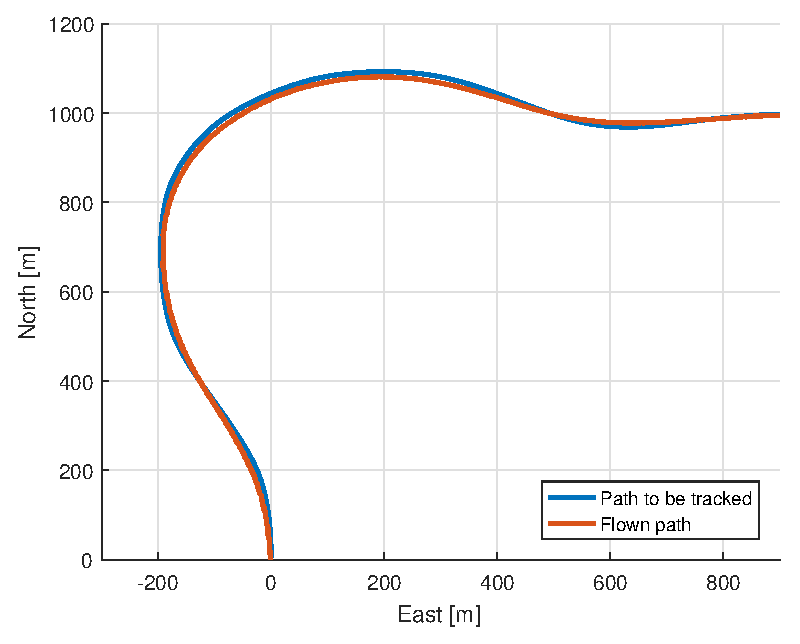
\includegraphics[width=0.8\textwidth, keepaspectratio=true]{../../results/sim/easy_path/fig_lin/tracking.eps}}
	\caption{Result when tracking the optimized path.}
	\label{fig:sim_tracking}
\end{figure}

\import{/}{gentle_path.tex}